\documentclass[hyperref={colorlinks=true,linkcolor=blue,urlcolor=blue},numbers]{beamer}
\usepackage{amsmath,paunits,shortcuts,overpic}
%\usepackage[usenames]{color}
\setbeamertemplate{navigation symbols}{}
\setbeamertemplate
    {footline}
    {\quad\strut\insertsection
      \hfill\insertframenumber/\inserttotalframenumber\strut\quad} 

\graphicspath{{./figures/}}

\newcommand{\rad}{%
   \ensuremath{I}
}

\newcommand{\irrad}{%
   \ensuremath{F}
}


\newcommand{\zenith}{%
   \ensuremath{\theta}
}

\newcommand{\azimuth}{%
   \ensuremath{\phi}
}

\newcommand{\trans}{%
   \ensuremath{Tr}
}

\newcommand{\abs}{%
   \ensuremath{\alpha}
}


\newcommand{\volabs}{%
   \ensuremath{\beta}
}

\newcommand{\massabs}{%
   \ensuremath{\kappa}
}

\begin{document}

\begin{frame}
  \frametitle{ Introduction}

  \begin{itemize}


  \item  Reading:  Stull 224-226, W\&H 134-136


  \item Questions:
    \begin{itemize}

  \item How do we handle an atmosphere that is not only absorbing, but emitting radiation?
  \item Major problem is that now temperature, absorptivity, emissivity and  transmisivity
are all changing with height
\item Major opportunity that if you know some of these quantities you can use remote sensing
to get others (like the temperature given the transmittance).
\item The approach:  from the Beer's law notes we know that absorption is maximum when
$\tau_\lambda = 1$.  It will turn out that emission is also maximum at $\tau_\lambda = 1$.
So by measuring radiance at several wavelengths we can get information about emission
at different optical depths.

    \end{itemize}

  \end{itemize}


\end{frame}

\begin{frame}
  \frametitle{ Example: High resolution infrared radiation sounder (HIRS): 12 IR channels}

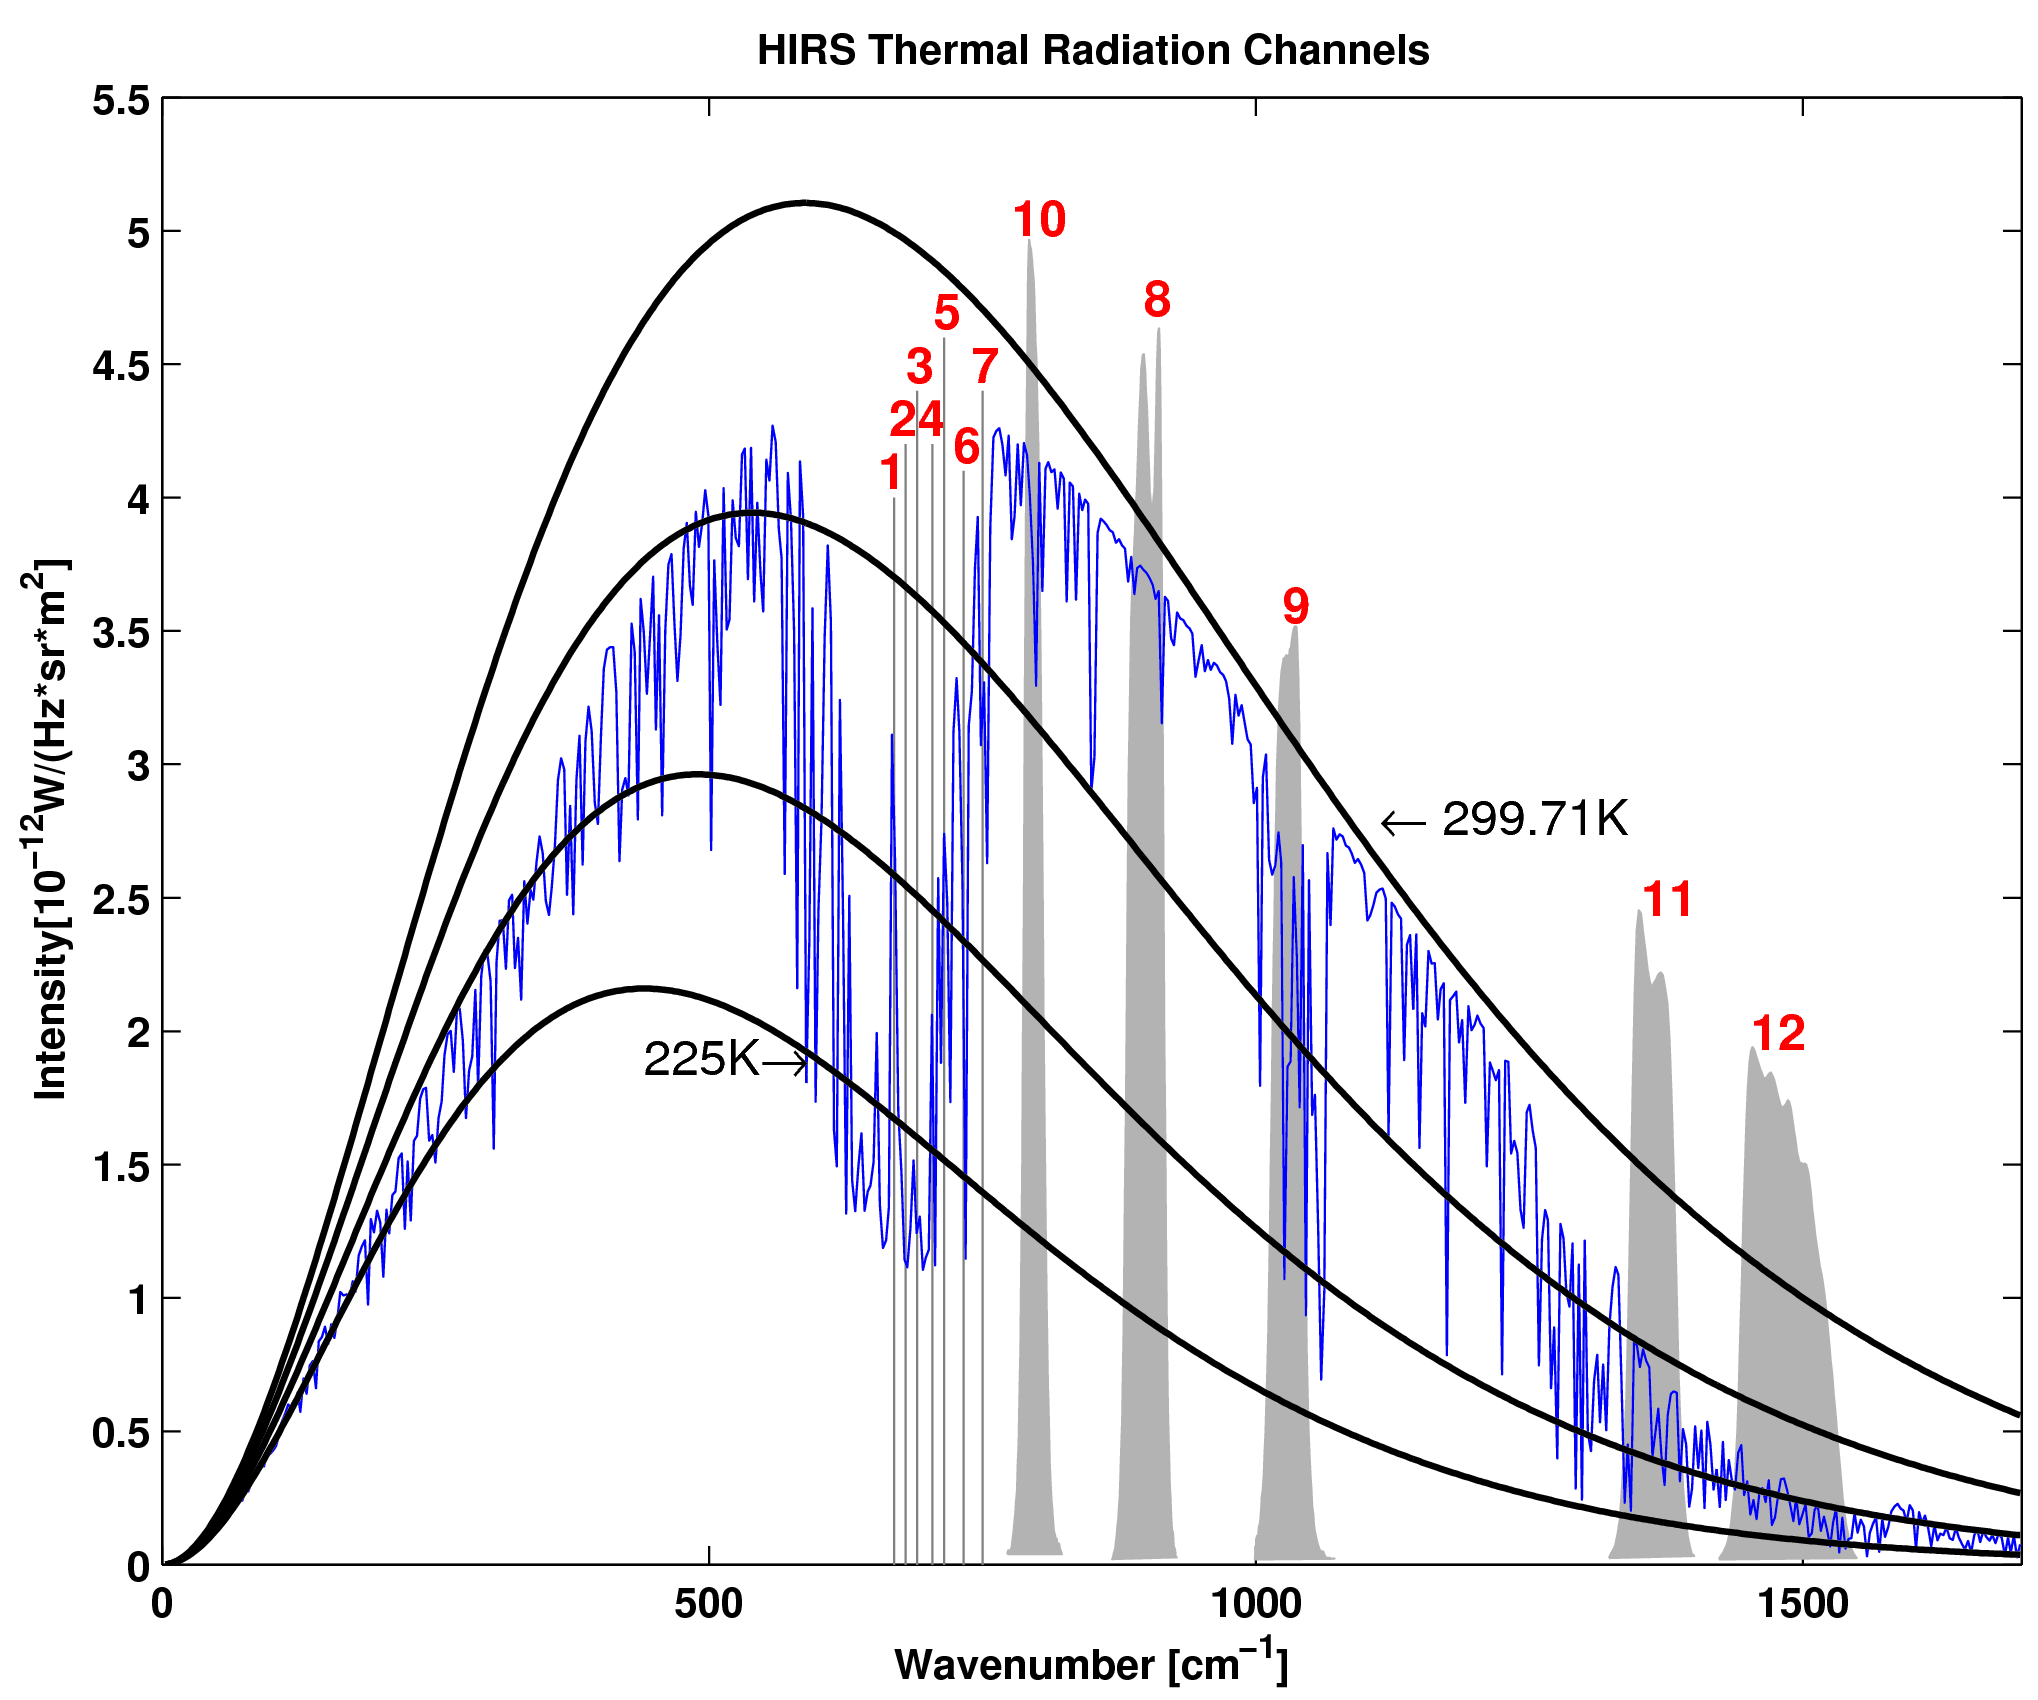
\includegraphics[width=0.8\textwidth]{planck1_full.png}
\end{frame}

\begin{frame}
  \frametitle{ HIRS weighting functions}

\begin{overpic}[tics=20,width=0.45\textwidth]{weightingfunctionfigs.png}
  \put(75,40){
     \begin{minipage}{0.5\textwidth}
         Using these 7 weighting functions we can invert 7 radiance measurements to find
a vertical profile of temperature in the atmosphere
     \end{minipage}
   }
\end{overpic}
 
\end{frame}


\begin{frame}
  \frametitle{First step: constant temperature layer}

\begin{itemize}

\item Review from Beers Law notes:


\item Review Beer's law, letting $\mu=\cos \theta$ and defining $\tau_\lambda$ increasing upward:

  \begin{gather}
d I_\lambda = -I_\lambda  \rho_{air} r_{gas} k_\lambda ds  = -I_\lambda  \rho_{air} r_{gas} k_\lambda dz/\mu  = -I_\lambda d\tau_\lambda /\mu \label{eq:beers}\\
\text{Now use $d\tau_\lambda/\mu = \rho_{air} r_{gas} dz/\mu$ and integrate} \nonumber\\
\text{ from $(I_{\lambda 0}, 0)$ to$ (I_{\lambda}, \tau{_\lambda})$} \nonumber\\
\int_{I_{\lambda 0}}^{I_\lambda}  \frac{d I^\prime_\lambda}{I^\prime_\lambda} =\int_{I_{\lambda 0}}^{I_\lambda} d\ln I^\prime_\lambda 
  = - \int_0^{\tau_\lambda} d\tau^\prime_\lambda/\mu \nonumber\\
\left . \ln I^\prime_\lambda \right |_{I_{\lambda 0}}^{I_\lambda} = \ln \left [ \frac{I_\lambda}{I_{\lambda 0}} \right ]
  = - \int_0^{\tau_\lambda} d\tau^\prime_\lambda/\mu = - \tau_\lambda/\mu  \nonumber\\
\text{and taking $\exp$ of both sides gives:} \nonumber \\
  I_{\lambda} = I_{\lambda 0} \exp ( - \tau_\lambda/\mu ) \nonumber
  \end{gather}


\end{itemize}

\end{frame}


\begin{frame}
  \frametitle{absorptivity, emissivity, transmissivity}

\begin{itemize}



\item Remember the relationships between 
$Tr_\lambda$, $\tau_\lambda$, $\alpha_\lambda$ and $\epsilon_\lambda$:
  \begin{gather*}
Tr_\lambda = \frac{I_{\lambda}}{I_{\lambda 0}} = \exp ( - \tau_\lambda/\mu ) \\
\text{and if $\tau_\lambda \ll 1$ then you can use a Taylor expansion}:\\
i.e. \exp(-\tau_\lambda/\mu) \approx (1 -\tau_\lambda/\mu) \\
  d Tr_\lambda = d \exp(-\tau_\lambda/\mu) = - \exp(-\tau_\lambda/\mu)\, d\tau_\lambda/\mu \, \approx\\
 \, - (1 -\tau_\lambda/\mu)\, d\tau_\lambda/\mu
 \, \approx \,- d\tau_\lambda/\mu\\
\text{or do the expansion first then take the differential: } \\
  d Tr_\lambda = d \exp(-\tau_\lambda/\mu) \approx  d(1 -\tau_\lambda/\mu)
=  - d\tau_\lambda/\mu\\
\text{conservation of energy without reflection says:}\\
  Tr_\lambda + \alpha_\lambda =1 \\
  dTr_\lambda = - d\alpha_\lambda\\
  d\alpha_\lambda \approx d\tau_\lambda/\mu
  \end{gather*}


\end{itemize}

\end{frame}

\begin{frame}
  \frametitle{Schwartzchild equation}

  \begin{itemize}
  \item We want to derive Stull equation 8.3 and 8.4 on pages 224 and 225 (W\&H 4.42)
that give the radiance for an atmosphere that is not only absorbing, but emitting radiation.
This is called the ``Schwartzchild equation''

\item Start with figuring out how the emissivity is related to the optical depth
using Kirchoff's law.

  \end{itemize}
\end{frame}

\begin{frame}
  \frametitle{ Kirchoff's law and the Schwartzchild equation}

  \begin{itemize}
  \item Kirchoff says $\epsilon_\lambda = \alpha_\lambda$ so:
    \begin{equation*}
      d\epsilon_\lambda =  d\alpha_\lambda=d\tau_\lambda/\mu
    \end{equation*}

  \item So the radiance gain due to emission is:

    \begin{equation*}
  \label{eq:emission}
  d\rad_\lambda^{emission} = d\epsilon_\lambda B_\lambda (T) = \kappa_\lambda \rho_g  B_\lambda (T) dz/ \mu = B_\lambda(T) d \tau_\lambda /\mu
    \end{equation*}


  \item and combine this with the absorption loss (\ref{eq:beers}) to get \textit{Schwartzchild's equation} (W\&H  4.41)

\begin{gather*}
  \label{eq:schwart2}
   d\rad_\lambda = -\rad_\lambda\, d\tau_\lambda/\mu + B_\lambda (T)\, d\tau_\lambda/\mu \\
  \mu \frac{d\rad_\lambda}{d\tau_\lambda} = -\rad_\lambda + B_\lambda (T)
\end{gather*}


  \end{itemize}

\end{frame}

\begin{frame}
  \frametitle{ Schwartzchild, cont.}

  \begin{itemize}
  \item In class we derived the following:
 if the temperature $T_{atm}$ (and hence $B_\lambda(T_{atm})$) is constant with height

\begin{equation}
  \label{eq:constTb}
  \int_{\rad_{\lambda 0}}^{\rad_\lambda} \frac{d\rad^\prime_\lambda}{\rad^\prime_\lambda -
  B_\lambda} = - \int_0^{\tau_\lambda} d\tau^\prime_\lambda / \mu
\end{equation}

\begin{equation}
  \label{eq:constTc}
  \ln \left (\frac{\rad_\lambda - B_\lambda}{\rad_{\lambda 0} - B_\lambda}
  \right ) = - \tau_\lambda / \mu
\end{equation}

\begin{gather}
  \label{eq:constTd}
  \rad_\lambda - B_\lambda = (\rad_{\lambda 0} - B_\lambda) \exp(-\tau_\lambda
  / \mu)) \\
\text{where } \mu=\cos \zenith \nonumber\\
\text{or rearranging:}\nonumber\\
  \rad_\lambda = \rad_{\lambda 0} \exp( -\tau_\lambda /\mu ) + B_\lambda (T_{atm})(1
  - \exp( -\tau_\lambda / \mu))
\end{gather}



  \end{itemize}

\end{frame}

\begin{frame}
  \frametitle{What the equation is saying:}

  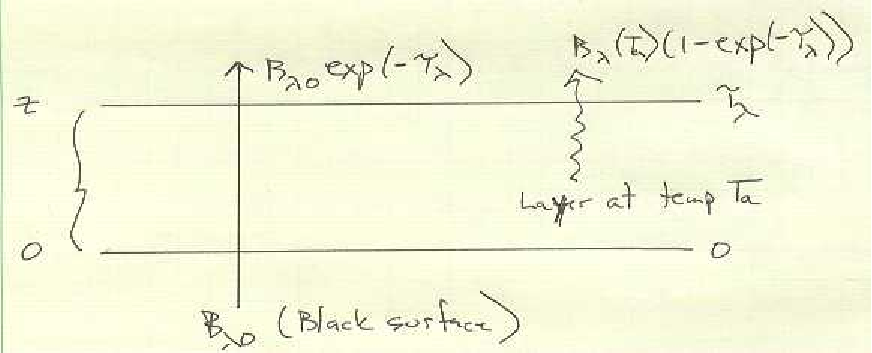
\includegraphics[width=\textwidth]{fig_isothermal}

  \begin{itemize}
  \item If we set $\mu=1$ (straight up) and define:

    \begin{gather*}
  \trans_\lambda = \exp( -\tau_\lambda
/\mu ) = 1 - \mathrm{absorption} = 1 - \abs_\lambda \\
        \epsilon_\lambda = (1 - \exp( -\tau_\lambda / \mu))\\
\text{then we're back to lecture 8, slide II.2 for a one layer atmosphere}\\
  \rad_\lambda = \rad_{\lambda 0} Tr_\lambda(\tau_\lambda ,\mu ) + B_\lambda (T_{atm}) \epsilon_\lambda
    \end{gather*}

\end{itemize}
\end{frame}

\begin{frame}
  \frametitle{A subtle problem: }

  \begin{itemize}
  \item It looks like we've got a paradox.  On the last slide I said that integrating the transmission
over $\tau_\lambda$ gives:

    \begin{equation}
\label{eq:true}
              \epsilon_\lambda = (1 - \exp( -\tau_\lambda / \mu))
    \end{equation}


  \item But I also said that Kirchoff's law tells us that:

    \begin{equation*}
            d\epsilon_\lambda =  d\alpha_\lambda=d\tau_\lambda/\mu
    \end{equation*}

which, if I integrate gives 

    \begin{equation}
\label{eq:false}
              \epsilon_\lambda = \tau_\lambda/\mu
    \end{equation}

How can (\ref{eq:true}) and (\ref{eq:false}) both be right?


  \end{itemize}

\end{frame}

\begin{frame}
  \frametitle{ The answer}

  \begin{itemize}
  \item To see where the difference comes from, go back to conservation of energy:

    \begin{gather}
        Tr_\lambda + \alpha_\lambda =1 \\
  dTr_\lambda = - d\alpha_\lambda = - d\epsilon_\lambda \label{eq:exact}\\
  d\alpha_\lambda \approx d\tau_\lambda/\mu \label{eq:third}
    \end{gather}

Equation (\ref{eq:third}) involves the approximation that 

\begin{equation*}
    d Tr_\lambda = d \exp(-\tau_\lambda/\mu) \approx  d(1 -\tau_\lambda/\mu)
\end{equation*}
which is true as long as $\tau_\lambda \ll 1$

 If we integrate (\ref{eq:exact}) without this approximation to get the right $\epsilon_\lambda$:

\begin{equation*}
\int_0^{\epsilon_\lambda} d\epsilon_\lambda^\prime = \epsilon_\lambda =
-\int_0^{\tau_\lambda}    d \exp(-\tau^\prime _\lambda/\mu)  = 1 - \exp(\tau_\lambda/\mu) = 1 - Tr_\lambda
\end{equation*}


  \end{itemize}
\end{frame}
\begin{frame}
  \frametitle{ The answer, cont.}

  \begin{itemize}

  \item In words, the differential version of Kirchoff's law assumes that you are working with
a layer of very small transmissivity (i.e. extremely thin).   When you integrate
a thicker layer, you are adding small increments of $d \tau_\lambda$ to a layer
that has some finite optical depth.

\item   Trying to apply the infinitesmal approximation
to this thicker layer doesn't work, 
and you can't use the Taylor series approximation, which assumes
$\tau_\lambda \ll 1$.  


\item  (Picture to be placed here).


\item As long as you remember the difference between finite and infinitesimal layers, there's
no conflict.

  \end{itemize}


Next step: let temperature change with height.

\end{frame}

\end{document}

% ------------------------------------------------------------------------
% Sascha Frank

% Last modified: Thu Oct 6 10:37:34 MEST 2005



%   \frame{
%   \frametitle{Cloud histograms, 2003-2005 }
%   \begin{columns}
%   \begin{column}[b]{5cm}
%   \includegraphics[width=1.65in]{kubarfig2a.jpg}
%   \end{column}
%   \begin{column}[b]{5cm}
% \small{Optical depth/cloud top temperature histograms in the Western, Central and Eastern Pacific (\small{Kubbar et al., 2007})}\\
% $~$\\
% $~$\\
%   \includegraphics[width=1.65in]{kubarfig2b.jpg}
%   \end{column}
%   \end{columns}}




